\documentclass[beamer, en, version=2.0]{huangfusl-template}
\usepackage[scheme=plain]{ctex}
\usepackage{listings}
\usepackage{libertine}
\usepackage[normalem]{ulem}
\usefonttheme[onlymath]{serif}
% Change tt font to Source Code Pro
\usepackage{sourcecodepro}
\lstset{
    basicstyle=\ttfamily\footnotesize,
    backgroundcolor=\color{darkblue!10},
    % Set color paddings
    frame=single,
    framerule=0pt,
    breakatwhitespace=true,
    showstringspaces=false,
    % Set comment to gray and italic
    commentstyle=\color{gray}\itshape,
    % Set keyword to bold and darkblue
    keywordstyle=\color{darkblue}\bfseries,
    % Set string to darkred
    stringstyle=\color{darkred},
}

\setbeamertemplate{footline}{
    \begin{beamercolorbox}[colsep=1.5pt]{upper separation line foot}
    \end{beamercolorbox}
    \begin{beamercolorbox}[ht=2.5ex,dp=1.125ex,leftskip=.3cm,rightskip=.3cm plus1fil]{author in head/foot}
        {
            \usebeamerfont{author in head/foot}\insertshortauthor
        }
        \hfill
        {
            \url{https://github.com/HuangFuSL/python-lec}
        }
    \end{beamercolorbox}
    \begin{beamercolorbox}[ht=2.5ex,dp=1.125ex,leftskip=.3cm,rightskip=.3cm plus1fil]{title in head/foot}
        {
            \usebeamerfont{title in head/foot}\insertshorttitle
        }
        \hfill
        {
            \usebeamerfont{frame number}
            \usebeamercolor[fg]{frame number}
            \insertframenumber~/~\inserttotalframenumber
        }
    \end{beamercolorbox}
    \begin{beamercolorbox}[colsep=1.5pt]{lower separation line foot}
    \end{beamercolorbox}
}

\title[Lecture 1: Introduction to Python]{\LARGE{清华经管博士生工作坊}\newline\newline \large{Lecture 1: Introduction to Python}}
\author{皇甫硕龙}
\date{2024-04-18}
\splitsections

\begin{document}
    \begin{frame}[fragile]
        \maketitle
    \end{frame}
    \begin{frame}
        \frametitle{History of Python}

        Python is a high-level, \textbf{interpreted}, and general-purpose programming language. It was created by Guido van Rossum and first released in 1991.

        Currently, Python has two major versions: Python 2 and Python 3. Python 2 has reached its end of life on January 1, 2020. Python 3 is the future of Python and is under active development.
    \end{frame}
    \section{Installation}
    \begin{frame}[fragile]
        \frametitle{Install Python (Windows)}

        For Windows, the official download link of Python is: {\footnotesize \url{www.python.org/downloads/}}. Choose {\color{darkblue} Windows installer (64-bit)}.

        \only<1>{
        \begin{figure}
            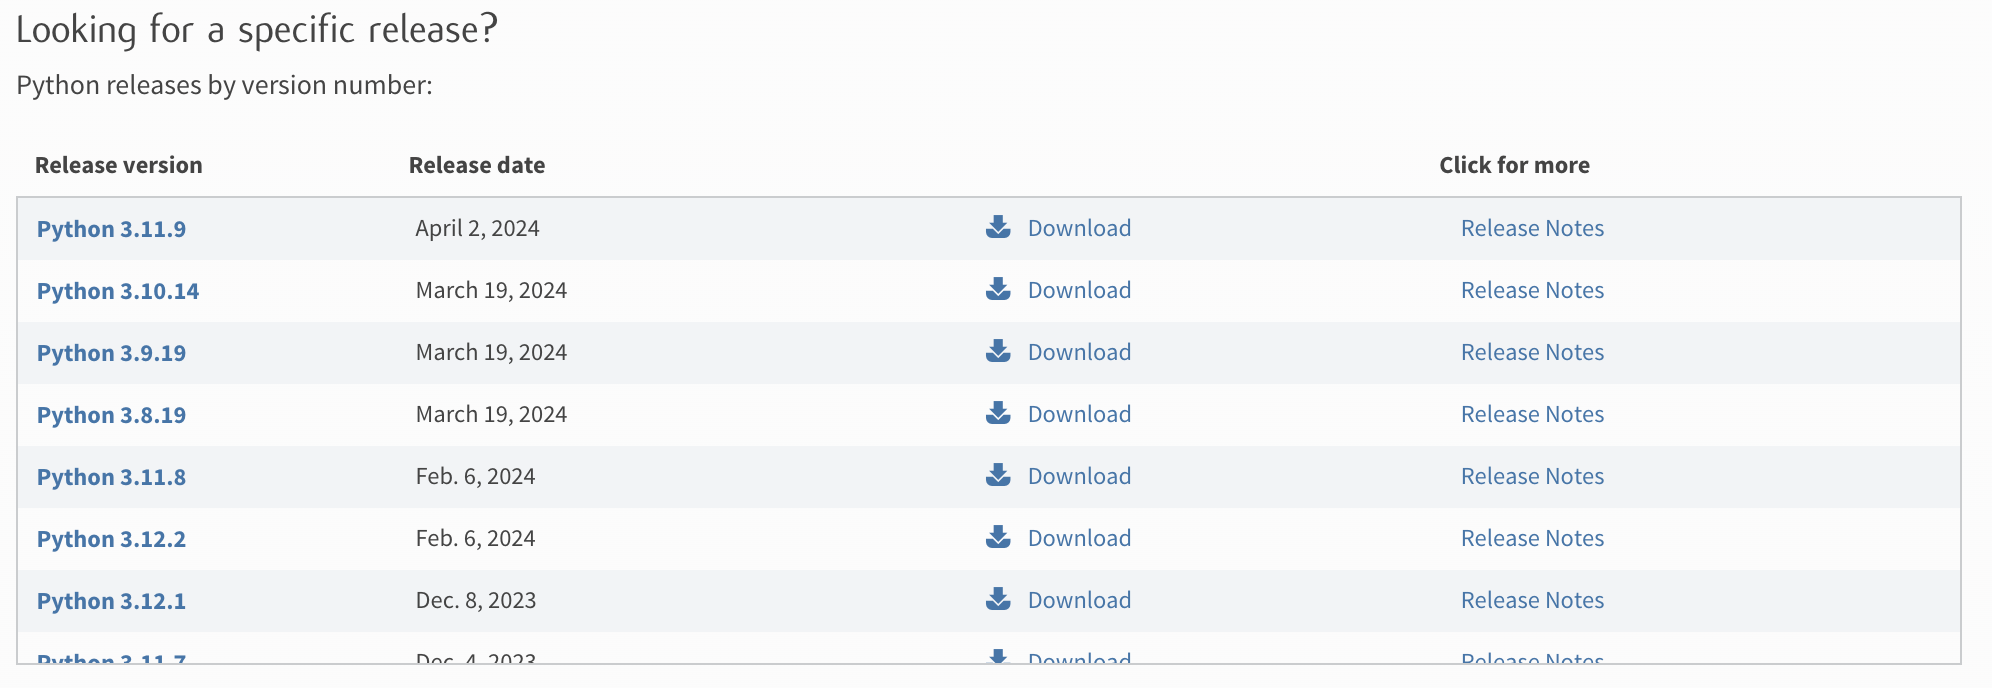
\includegraphics[width=0.8\linewidth]{imgs/1.png}
        \end{figure}
        }
        \only<2->{\addtocounter{framenumber}{1}}
        \only<2>{
        \begin{figure}
            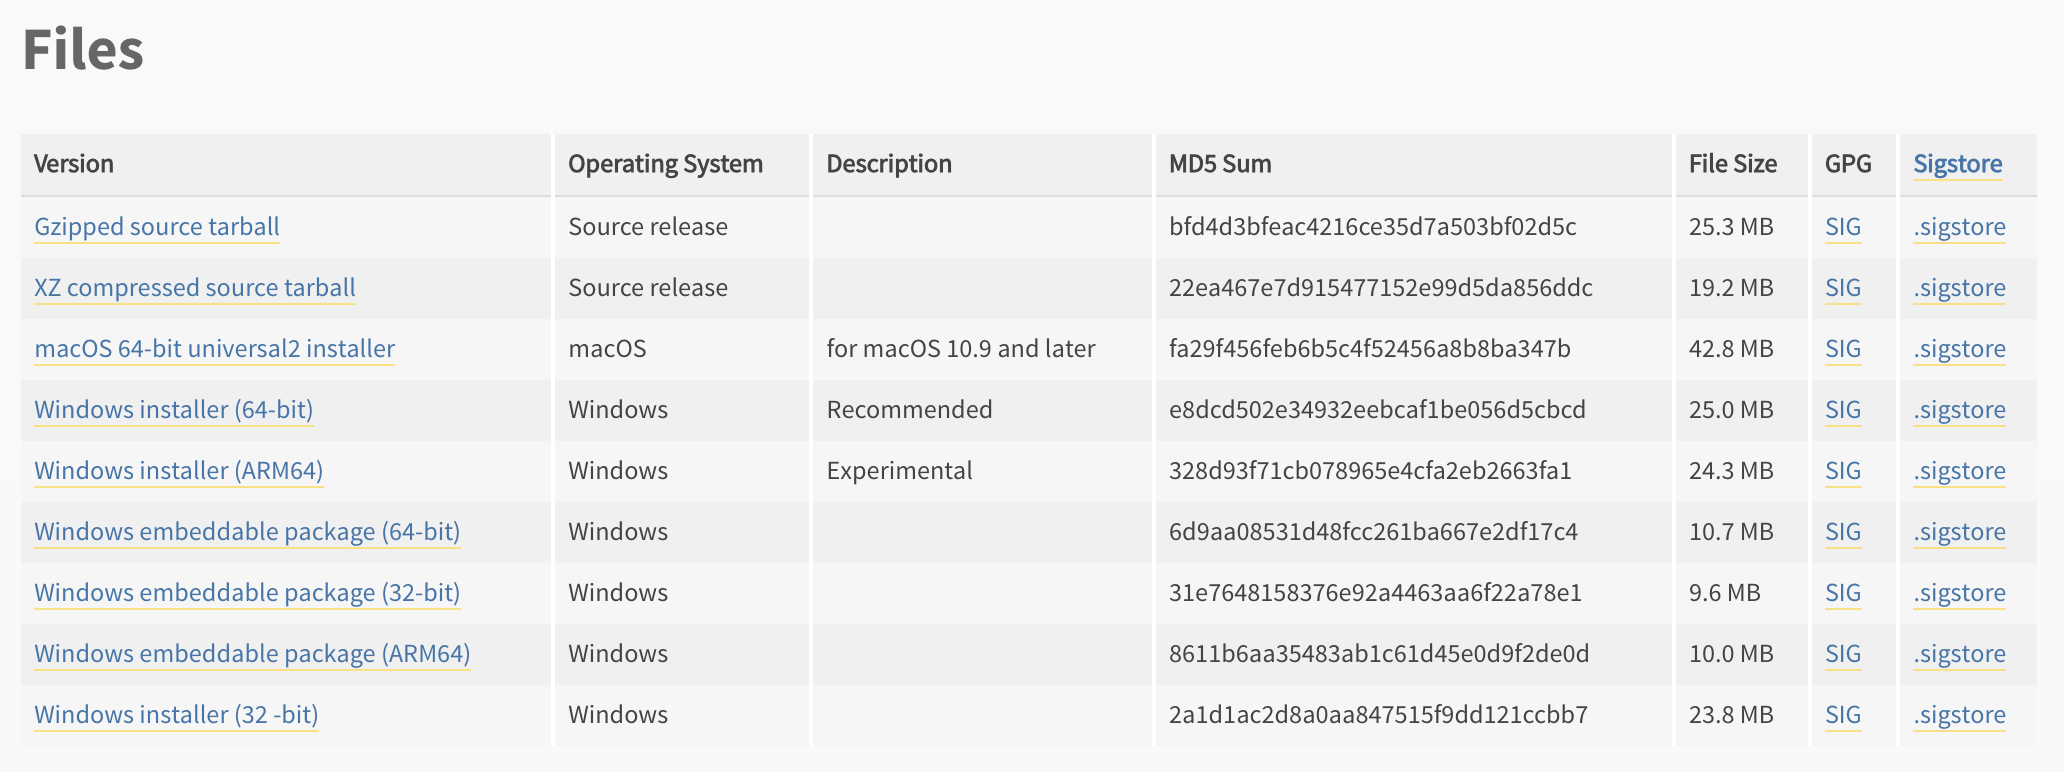
\includegraphics[width=0.8\linewidth]{imgs/2.png}
        \end{figure}
        }
        \only<3>{
        \begin{figure}
            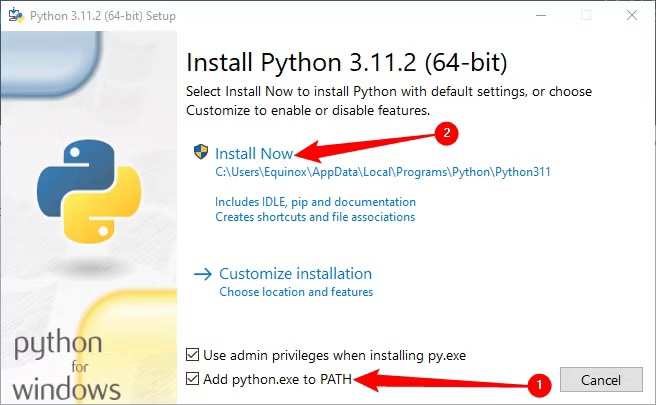
\includegraphics[width=0.6\linewidth]{imgs/3.jpg}
        \end{figure}
        }
    \end{frame}
    \begin{frame}[fragile]
        \frametitle{Install Python (macOS \& Linux)}

        For macOS users, you can use \href{https://github.com/Homebrew/install}{\color{darkblue} Homebrew} to install Python. Execute the following command in terminal:

        \begin{lstlisting}[language=bash]
brew install python
        \end{lstlisting}

        The installation command for Linux depends on the distribution. For Debian-based distributions, use:

        \begin{lstlisting}[language=bash]
sudo apt-get install python3 python3-pip
        \end{lstlisting}

    \end{frame}
    \begin{frame}[fragile]
        \frametitle{Verify Installation \& Install Packages}

        Notice that Python 2 and Python 3 are slightly different in syntax. Use {\footnotesize\verb|python3|} in terminal to ensure Python 3.

        \begin{lstlisting}[language=bash]
python3 --version # Check Python version
# Python 3.11.7
        \end{lstlisting}

        Use {\footnotesize\verb|pip3|} to install packages. {\color{darkred} Switch to \href{https://mirrors.tuna.tsinghua.edu.cn/help/pypi/}{Tsinghua pypi mirror} to speed up installation}.

        \begin{lstlisting}[language=bash]
# Set Tsinghua pypi mirror
pip3 config set global.index-url https://pypi.tuna.tsinghua.edu.cn/simple
# Install packages
pip3 install <package-name>
        \end{lstlisting}

    \end{frame}
    \begin{frame}
        \frametitle{Anaconda}

        Anaconda is a popular distribution of Python and R programming languages. It includes many packages for data science, machine learning, and scientific computing. And supports swiftly switching between different Python versions and environments.

        Refer to \href{https://zhuanlan.zhihu.com/p/25198543}{\color{darkblue} this ZhiHu article} for installation instructions and its usage.
    \end{frame}
    \begin{frame}[fragile]
        \frametitle{Python Interpreter}

        The installed {\footnotesize\verb|python3|} is an \textbf{interactive interpreter}. You can type and execute Python code directly in terminal.

        \begin{lstlisting}[breaklines]
Python 3.11.7 (main, Dec  4 2023, 18:10:11) [Clang 15.0.0 (clang-1500.1.0.2.5)] on darwin
Type "help", "copyright", "credits" or "license" for more information.
>>> print('Hello World!')
Hello World!
>>>
        \end{lstlisting}

        There are other interactive interpreters like {\footnotesize\verb|ipython|}.
    \end{frame}
    \begin{frame}[fragile]
        \frametitle{Execute Python Scripts}

        Python scripts are named with {\footnotesize\verb|.py|} suffix. We can run the script in terminal.

        \begin{lstlisting}[language=bash]
python3 script.py
        \end{lstlisting}

        Some packages (including {\footnotesize\verb|pip|}) are executable, use {\footnotesize\verb|-m <package>|} option to invoke the package.

        \begin{lstlisting}[language=bash]
python3 -m pip install numpy # Same as pip3 install numpy
        \end{lstlisting}
    \end{frame}
    \begin{frame}[fragile]
        \frametitle{Notebooks}

        Jupyter Notebook provides a convenient way to write and execute Python code. It is widely used in data analysis and machine learning.

        To use Jupyter Notebook, first install {\footnotesize\verb|jupyter|} package. Then execute the {\footnotesize\verb|jupyter notebook|} command in terminal. A browser window will spawn.
    \end{frame}
    \begin{frame}
        \frametitle{IDE for Python}

        We'll use \textbf{Visual Studio Code} as the IDE for Python programming. It is lightweight and supports various programming languages. Download from \href{https://code.visualstudio.com/download}{\color{darkblue} official website}.

        Search and install the \textbf{Python} extension in the \textbf{Extensions} tab. The extension provides syntax highlighting, code completion, and debugging support.
    \end{frame}
    \begin{frame}[fragile]
        \frametitle{External Resources}

        Here are external resources for Python programming. Remember to use them when you encounter problems.

        \begin{itemize}
            \item \href{https://docs.python.org/3/}{\color{darkblue} Official Python documentation}
            \item \href{https://www.stackoverflow.com/}{\color{darkblue} Stack Overflow}
            \item \href{https://chat.openai.com/}{\color{darkblue} ChatGPT} (although may not be accurate)
            \item \href{https://github.com/features/copilot}{\color{darkblue} GitHub Copilot} from \href{https://education.github.com/discount_requests/application}{\color{darkblue} GitHub Student Developer Pack}
            \item \href{https://www.csdn.net/}{\color{darkred}\sout{CSDN}}
        \end{itemize}

        Refer to the package documentation for package-specific problems.
    \end{frame}
    \section{Basic Python Syntax}
    \subsection{Use Python as a Calculator}
    \begin{frame}[fragile]
        \frametitle{Use Python as a Calculator}

        \begin{block}{Note}
            If a line starts with {\footnotesize\verb|>>>|}, it means that the line is executed in the interactive shell. If the expression has a non-{\footnotesize\verb|None|} result, it will be displayed after the expression.
        \end{block}

        We can use Python interpreter as an calculator and perform arithmetic operations. Also, we can call built-in functions by their names.

\begin{lstlisting}[language=python]
>>> 2 + 2
4
>>> 50 - 5 * 6
20
>>> print('Hello World!') # Function call
Hello World!
>>> x = 4 # Assign value to a variable
\end{lstlisting}
    \end{frame}
    \subsection{Identifiers}
    \begin{frame}[fragile]
        \frametitle{Storing Values}

        \textbf{Variables} are used to store some values. Use {\footnotesize\verb|=|} to assign a value to a variable. After assigning a value to a variable, we can use the variable to reference the value.

        \begin{block}{Note}
            Variables \textit{must} be assigned before referencing its value. Unlike C or C++, we do not need to declare the type of a variable.

\begin{lstlisting}[language=python]
>>> b
Traceback (most recent call last):
    File "<stdin>", line 1, in <module>
NameError: name 'b' is not defined
\end{lstlisting}
        \end{block}
    \end{frame}
    \begin{frame}[fragile]
        \frametitle{Identifiers}

        Identifier is the name of \textbf{variables} (or functions, classes, etc.) in Python. It can contain letters, digits, and underscores {\color{darkblue}\footnotesize\verb|_|}, but cannot start with a digit.

        \begin{lstlisting}[language=python]
# Valid identifiers
var, VAR, _var, var_1, _1, _
# Invalid identifiers
1var, var-1, var@1, var.1
        \end{lstlisting}

        \begin{block}{Note}
            Identifiers are case-sensitive. {\footnotesize\verb|var|} and {\footnotesize\verb|Var|} are different identifiers.
        \end{block}
    \end{frame}
    \begin{frame}[fragile]
        \frametitle{Reserved Words}

        Some words are reserved for special purposes in Python. They \textbf{cannot} be used as identifiers.

        \begin{lstlisting}[language=python, breaklines, breakautoindent=false, breakindent=0pt]
>>> import keyword
>>> keyword.kwlist
['False', 'None', 'True', 'and', 'as', 'assert', 'async', 'await', 'break', 'class', 'continue', 'def', 'del', 'elif', 'else', 'except', 'finally', 'for', 'from', 'global', 'if', 'import', 'in', 'is', 'lambda', 'nonlocal', 'not', 'or', 'pass', 'raise', 'return', 'try', 'while', 'with', 'yield']
        \end{lstlisting}
    \end{frame}
    \begin{frame}[fragile]
        \frametitle{``Soft'' Reserved Words}

        Python provides multiple built-in functions. If we assign value to them, the built-in functions will be shadowed. It is not recommended to use built-in functions as identifiers.

\begin{lstlisting}[language=python]
>>> print('Hello World!')
Hello World!
>>> print = 'Hello World!' # Assign value to print
>>> print('Hello World!')
Traceback (most recent call last):
    File "<stdin>", line 1, in <module>
TypeError: 'str' object is not callable
\end{lstlisting}
    \end{frame}
    \subsection{Miscellaneous}
    \begin{frame}[fragile]
        \frametitle{Statements}

        A statement is a single line of code that performs some action. Python does not require semicolons {\footnotesize\verb|;|} to end a statement.

        \begin{enumerate}
            \item \textbf{Expression statement}: Evaluates an expression.
            \item \textbf{Assignment statement}: Assigns the value of an expression to a variable. Here {\footnotesize\verb|=|} should be read as ``is assigned'' ($\leftarrow$).
\begin{lstlisting}[language=python]
x = 10
y = 4 * x + 3
\end{lstlisting}
\begin{lstlisting}[language=python]
print('Hello World!')
x * 3 + y * 2
\end{lstlisting}
        \end{enumerate}
    \end{frame}
    \begin{frame}[fragile]
        \frametitle{Code Blocks}

        Code blocks are a group of statements that are executed together. In Python, code blocks are defined by \textbf{indentation}. We can use \textbf{4 spaces} or \textbf{1 tab} to indent, but we should not mix them in one statement.

\begin{lstlisting}[language=python, showspaces=true, showstringspaces=true]
if x > 0:
    x += 1
    print('Positive')
else:
    x -= 1
    print('Non-positive')
\end{lstlisting}
    \end{frame}
    \begin{frame}[fragile]
        \frametitle{Comments}

        Comments are used to explain the code. In Python, comments start with a {\footnotesize\verb|#|}. Any text after the {\footnotesize\verb|#|} is ignored by the Python interpreter.

        Under certain circumstances, \textbf{docstrings} wrapped by triple quotes {\footnotesize\verb|'''|} or {\footnotesize\verb|"""|} are used to document functions or modules.

\begin{lstlisting}[language=python]
# This is a comment
x = 10 # This is also a comment
def func():
    '''This is a docstring'''
    pass
\end{lstlisting}
    \end{frame}
    \begin{frame}[fragile]
        \frametitle{Line Continuation}

        When a line is too long, we can use a backslash {\footnotesize\verb|\|} to split the line. The backslash must be the last character on the line. If the backslash is after a {\footnotesize\verb|#|}, the backslash is considered as a part of comment.

\begin{lstlisting}[language=python]
x = 1 + 2 + 3 + 4 + 5 + \
    6 + 7 + 8 + 9 + 10
# x = 55
\end{lstlisting}

        {\footnotesize\itshape\textbf{Remark:} If the line is inside parentheses, brackets, or braces, we can split the line without a backslash.}
    \end{frame}
    \section{Data Structures}
    \subsection{Basic Data Types}
    \begin{frame}[fragile]
        \frametitle{Basic Data Types}

        Python has several built-in data types, including \textbf{integers} ({\footnotesize\verb|int|}), \textbf{floating-point numbers} ({\footnotesize\verb|float|}), \textbf{strings} ({\footnotesize\verb|str|}), \textbf{booleans} ({\footnotesize\verb|bool|}), and container types like \textbf{lists} ({\footnotesize\verb|list|}), \textbf{tuples} ({\footnotesize\verb|tuple|}), and \textbf{dictionaries} ({\footnotesize\verb|dict|}), \textbf{sets} ({\footnotesize\verb|set|}). {\footnotesize\verb|None|} is a special type representing \textbf{null}.

        Basic types are \textbf{immutable}, while most container types except \textbf{frozenset} and \textbf{tuple} are \textbf{mutable}.
    \end{frame}
    \begin{frame}[fragile]
        \frametitle{Integers}

        \textbf{Integers} are whole numbers without a decimal point. They can be positive or negative. In Python, integers have unlimited range. Underscores {\footnotesize\verb|_|} can be used to separate digits for readability.

\begin{lstlisting}[language=python]
dec = 123
neg = -456
big = 123456789012345678901234567890
underscore = 1_000_000 # Underscores for readability
hex_ = 0x10 # Hexadecimal number starts with 0x
oct_ = 0o10 # Octal number starts with 0o
bin_ = 0b10 # Binary number starts with 0b
\end{lstlisting}
    \end{frame}
    \begin{frame}[fragile]
        \frametitle{Floating-point numbers}

        \textbf{Floating-point numbers} (or floats) are numbers \textbf{with a decimal point}. For example, {\footnotesize\verb|1|} is an integer and  {\footnotesize\verb|1.0|} is a float. They can be positive or negative. \textbf{NaN} (Not a Number) and \textbf{Infinity} are also floating-point numbers.

\begin{lstlisting}[language=python]
pi = 3.14159
neg_e = -2.71828
sci = 1.23e-4 # Scientific notation
nan = float('nan') # Not a Number
inf = float('inf') # Infinity
\end{lstlisting}

{\color{darkred}In Python, floating-point numbers are not precise.}
\begin{lstlisting}[language=python]
>>> 0.1 + 0.2
0.30000000000000004
\end{lstlisting}
    \end{frame}
    \begin{frame}[fragile]
        \frametitle{Strings}

        \textbf{Strings} are sequences of characters. They are enclosed in single quotes {\footnotesize\verb|'|}, double quotes {\footnotesize\verb|"|}, or triple quotes {\footnotesize\verb|'''|} and {\footnotesize\verb|"""|}. Strings quoted by single quotes and double quotes do not allow line breaks.

        When two \textbf{quoted} strings are adjacent, they are concatenated.

\begin{lstlisting}[language=python]
s1 = 'Hello' # Single quotes
s2 = "World" # Double quotes
s3 = '''Hello
World''' # Triple quotes allows multi-line strings
s4 = 'Hello' 'World' # Concatenation
\end{lstlisting}
    \end{frame}
    \begin{frame}[fragile]
        \frametitle{Escape Characters}

        Some characters are not allowed to be directly written in strings. We need to use \textbf{escape characters} to represent them.

        \begin{table}[h]
            \begin{tabular}{ccc}
                \toprule
                Description & Character & Escape Sequence \\
                \midrule
                Single quote & {\footnotesize\verb|'|} & {\footnotesize\verb|\'|} \\
                Double quote & {\footnotesize\verb|"|} & {\footnotesize\verb|\"|} \\
                Backslash & {\footnotesize\verb|\|} & {\footnotesize\verb|\\|} \\
                Newline & {\footnotesize\verb|\n|} & \\
                Tab & {\footnotesize\verb|\t|} & \\
                \bottomrule
            \end{tabular}
        \end{table}
    \end{frame}
    \begin{frame}[fragile]
        \frametitle{Raw Strings}

        If we do not want backslashes to be treated as escape characters, we can use \textbf{raw strings} by adding a prefix {\footnotesize\verb|r|} before the string.

        Notice that raw strings cannot end with a odd number backslash.

\begin{lstlisting}[language=python]
path = 'C:\\Users\\huangfusl\\Desktop' # Normal string
path = r'C:\Users\huangfusl\Desktop' # Raw string
path = r'C:\Users\huangfusl\Desktop\' # Invalid raw string
\end{lstlisting}
    \end{frame}
    \begin{frame}[fragile]
        \frametitle{Booleans}

        \textbf{Booleans} are binary values, either {\footnotesize\verb|True|} or {\footnotesize\verb|False|}. They are used to represent the truth value of an expression.

\begin{lstlisting}[language=python]
t = True
f = False
\end{lstlisting}
    \end{frame}
    \subsection{Operators}
    \begin{frame}[fragile]
        \frametitle{Operators}

        Python supports various operators, including \textbf{arithmetic operators}, \textbf{comparison operators}, \textbf{logical operators}, and \textbf{bitwise operators}. Some operators have the ``in-place'' version, like {\footnotesize\verb|+=|} and {\footnotesize\verb|-=|}.

    \end{frame}
    \begin{frame}[fragile]
        \frametitle{Arithmetic Operators}

        \textbf{Arithmetic operators} include addition {\footnotesize\verb|+|}, subtraction {\footnotesize\verb|-|}, multiplication {\footnotesize\verb|*|}, division {\footnotesize\verb|/|}, floor division {\footnotesize\verb|//|}, modulus {\footnotesize\verb|%|}, and exponentiation {\footnotesize\verb|**|}.

\begin{lstlisting}[language=python]
# Arithmetic operators
5 + 4 # Addition, 9
4.3 - 2 # Subtraction, 2.3
3 * 7 # Multiplication, 21
2 / 4 # Division, 0.5
2 // 4 # Floor division, 0
17 % 3 # Modulus, 2
2 ** 5 # Exponentiation, 32
\end{lstlisting}
    \end{frame}
    \begin{frame}[fragile]
        \frametitle{Comparison Operators}

        \textbf{Comparison operators} are used to compare two values. They return a \textbf{boolean} value. Comparison operators include {\color{darkred}\footnotesize\verb|==|}, {\footnotesize\verb|!=|}, {\footnotesize\verb|>|}, {\footnotesize\verb|<|}, {\footnotesize\verb|>=|}, and {\footnotesize\verb|<=|}.
    \end{frame}
    \begin{frame}[fragile]
        \frametitle{Logical Operators}

        \textbf{Logical operators} are used to combine multiple conditions. Logical operators include {\footnotesize\verb|and|}, {\footnotesize\verb|or|}, and {\footnotesize\verb|not|}.

\begin{lstlisting}[language=python]
# Logical operators
True and False # False
True or False # True
not True # False
\end{lstlisting}

        Variables other than binary values can be used in logical operators. In Python, \textbf{0}, \textbf{None}, and empty containers are considered \textbf{False}. Other values are considered \textbf{True}.

        {\footnotesize\itshape\textbf{Remark:} The logical operators are \textbf{short-circuit}, i.e. if the result can be determined by the first operand, the second operand will not be evaluated.}
    \end{frame}
    \begin{frame}[fragile]
        \frametitle{Bitwise Operators}

        \textbf{Bitwise operators} are used to perform bitwise operations on integers. Bitwise operators include {\footnotesize\verb|&|}, {\footnotesize\verb+|+}, {\footnotesize\verb|^|}, {\footnotesize\verb|~|}, {\footnotesize\verb|<<|}, and {\footnotesize\verb|>>|}.

        These operators are rarely used in daily programming. However, packages including \textbf{pandas} may use bitwise operators.
    \end{frame}
    \begin{frame}[fragile]
        \frametitle{In-place Operators}

        \textbf{In-place operators} are used to modify the value of a variable in place. They are the combination of arithmetic operators and assignment operators. All arithmetic operators and bitwise operators have in-place versions.

\begin{lstlisting}[language=python]
x = 10
x += 5 # Equivalent to x = x + 5
x *= 2 # Equivalent to x = x * 2
x /= 3 # Equivalent to x = x / 3
\end{lstlisting}
    \end{frame}
    \begin{frame}[fragile]
        \frametitle{Type Conversion}

        Python automatically converts data types when needed. We can also explicitly convert data types using type functions.

        \begin{itemize}
            \item {\footnotesize\verb|int()|}: Convert to integer. For floating-point numbers, it truncates the decimal part.
            \item {\footnotesize\verb|float()|}: Convert to float. Scientific notation is supported.
            \item {\footnotesize\verb|str()|}: Convert to string.
            \item {\footnotesize\verb|bool()|}: Convert to boolean. \textbf{0}, \textbf{None} and empty containers are \textbf{False}. Other values are \textbf{True}.
        \end{itemize}
\begin{lstlisting}[language=python]
int(3.14) # 3
float('3.14e2') # 314.0
str(3.14) # '3.14'
bool('false') # True
\end{lstlisting}
    \end{frame}
    \begin{frame}[fragile]
        \frametitle{Methods on Strings}

        Strings support various methods including {\footnotesize\verb|upper()|}, {\footnotesize\verb|lower()|}, {\footnotesize\verb|strip()|}, {\footnotesize\verb|split()|}, {\footnotesize\verb|join()|}, {\footnotesize\verb|replace()|}, {\footnotesize\verb|find()|}, {\footnotesize\verb|count()|}, and {\footnotesize\verb|startswith()|}.

        Usage of the above methods will be introduction in future slides.

        \begin{block}{Note}
            Since strings are immutable, if any method modifies the string, it will return a new string.
        \end{block}
    \end{frame}
    \subsection{Container Types}
    \begin{frame}[fragile]
        \frametitle{Container Types}

        \textbf{Container types} are used to store multiple values. The common container types in Python are \textbf{lists}, \textbf{tuples}, \textbf{dictionaries}, and \textbf{sets}. Container types can store values of different types.

        \begin{itemize}
            \item \textbf{Lists}: \textbf{Ordered}, \textbf{mutable} collection of items, represented by square brackets {\footnotesize\verb|[]|}.
            \item \textbf{Tuples}: \textbf{Ordered}, \textbf{immutable} collection of items, represented by parentheses {\footnotesize\verb|()|}.
            \item \textbf{Dictionaries}: \textbf{Unordered}, \textbf{mutable} collection of key-value pairs, represented by curly braces {\footnotesize\verb|{}|}.
            \item \textbf{Sets}: \textbf{Unordered}, \textbf{mutable} collection of \textbf{unique} items, represented by curly braces {\footnotesize\verb|{}|}.
            \item \textit{\textbf{Strings}}: strings can also be considered as a container type - a sequence of characters.
        \end{itemize}
    \end{frame}
    \begin{frame}[fragile]
        \frametitle{Breakdown of Container Types}

        Container types can be divided into multiple categories based on their properties.

        \begin{itemize}
            \item \textbf{Sequences} are ordered collections of items. Lists, tuples are sequences. Lists, tuples and strings are sequences.
            \item \textbf{Mapping} are collections of key-value pairs. Dictionaries are mappings.
            \item \textbf{Sets} are collections of unique items.
        \end{itemize}
    \end{frame}
    \begin{frame}[fragile]
        \frametitle{Lists}

        \textbf{Lists} are surrounded by square brackets {\footnotesize\verb|[]|}. They can contain any type of data, including other lists (nested lists). Lists are \textbf{mutable}. Empty lists are represented by {\footnotesize\verb|[]|}.

        List support arithmetic operations including concatenation {\footnotesize\verb|+|} and repetition {\footnotesize\verb|*|}.

\begin{lstlisting}[language=python]
nums = [1, 2, 3, 4, 5]
names = ['Alice', 'Bob', 'Charlie']
nested = [1, 'Alice', [2, 3]]
empty = []
add = nums + names # Concatenation
mul = names * 2 # Repetition
\end{lstlisting}
    \end{frame}
    \begin{frame}[fragile]
        \frametitle{Containers: Check Element Existence}

        Since containers hold multiple values. We can use {\footnotesize\verb|in|} and {\footnotesize\verb|not in|} to check if a value is in the container.

\begin{lstlisting}[language=python]
>>> 1 in [1, 2, 3]
True
>>> 0 in [1, 2, 3]
False
>>> 0 not in [1, 2, 3]
True
\end{lstlisting}


        {\footnotesize\itshape\textbf{Remark:} For dictionaries, the operator checks if the \textbf{key} is in the dictionary. For strings, it checks if the substring is in the string.}

    \end{frame}
    \begin{frame}[fragile]
        \frametitle{Sequences: Concatenation and Repetition}

        Sequences support using {\footnotesize\verb|+|} to concatenate two sequences and {\footnotesize\verb|*|} to repeat a sequence. When using {\footnotesize\verb|+|}, the two sequences must have the same type.

\begin{lstlisting}[language=python]
nums = [1, 2, 3]
names = ['Alice', 'Bob']
add = nums + names # [1, 2, 3, 'Alice', 'Bob']
mul = names * 2 # ['Alice', 'Bob', 'Alice', 'Bob']
error = nums + (1, 2, 3) # TypeError, cannot add tuple to list
\end{lstlisting}

        \begin{block}{Note}
            The two sequences are not modified in place. The result is a new sequence.
        \end{block}
    \end{frame}
    \begin{frame}[fragile]
        \frametitle{Sequences: Indexing Elements}

        For container types except sets, we can access elements by their index or key using square brackets {\footnotesize\verb|[]|}. {\color{darkred}The index starts from 0}. Negative indices are used to access elements from the end.

\begin{lstlisting}[language=python]
nums = [1, 2, 3, 4, 5]
scores = {'Alice': 90, 'Bob': 85, 'Charlie': 88}
nums[0] # 1
nums[-1] # 5
scores['Bob'] # 85
\end{lstlisting}

    If the key or index does not exist in the container, a {\footnotesize\verb|KeyError|} or {\footnotesize\verb|IndexError|} will be raised.

    \end{frame}
    \begin{frame}[fragile]
        \frametitle{Sequences: Slicing Elements}

        We can use \textbf{slicing} to access a subset of elements in a \textbf{ordered} container. Slicing is done by specifying the start index, end index, and step size separated by colons {\footnotesize\verb|:|}.

        \begin{block}{Note}
            \textbf{(1)} Indexing returns a single element, while slicing returns a subsequence of the same container type. \textbf{(2)} Slicing does not raise an error if the index is out of range. Only the valid part of the slice is returned. \textbf{(3)} The end index is exclusive.

            {\footnotesize\itshape\textbf{Remark:} Indexing on strings yields a string (of length 1).}
        \end{block}

\begin{lstlisting}[language=python]
nums = [1, 2, 3, 4, 5] # Indexes: 0, 1, 2, 3, 4
nums[:2] # Omit start index defaults to 0, [1, 2]
nums[3:] # Omit end index defaults to the end, [4, 5]
nums[:4:2] # [2, 3, 4] # Specify step size, [1, 3]
nums[::-1] # Negative step size reverses the result, [5, 4, 3, 2, 1]
\end{lstlisting}
    \end{frame}
    \begin{frame}[fragile]
        \frametitle{Methods on Sequences}

        Sequences support actions not changing the sequence in place, including {\footnotesize\verb|len()|}, {\footnotesize\verb|min()|}, {\footnotesize\verb|max()|}, {\footnotesize\verb|sum()|}. Sequences also have methods like {\footnotesize\verb|index()|}, {\footnotesize\verb|count()|}.

\begin{lstlisting}[language=python]
nums = [1, 2, 3, 4, 5]
len(nums) # Length of the list: 5
min(nums) # Minimum value: 1
max(nums) # Maximum value: 5
sum(nums) # Sum of the list: 15
nums.index(3) # Find the index of 3: 2
nums.count(3) # Count the number of 3: 1
\end{lstlisting}
    \end{frame}
    \begin{frame}[fragile]
        \frametitle{Mutable Sequences: Assignment on Indexes and Slices}

        Mutable container types (lists, dictionaries) support item assignment. We can assign a value to an index or a slice to change its elements.

\begin{lstlisting}[language=python]
nums = [1, 2, 3, 4, 5]
nums[2] = 10 # [1, 2, 10, 4, 5]
nums[2:4] = [1, 2, 3] # [1, 2, 1, 2, 3, 5]
\end{lstlisting}

        \begin{block}{Note}
            The length of the assigned value must match the length of the slice if step size is not 1.

\begin{lstlisting}[language=python]
nums = [1, 2, 3, 4, 5]
nums[2:4:2] = [1, 2, 3] # ValueError, nums[2:4:2] has length 1
\end{lstlisting}
        \end{block}
    \end{frame}
    \begin{frame}[fragile]
        \frametitle{Mutable Sequences: Extra Methods on Lists}

        Lists is mutable. Methods including {\footnotesize\verb|append()|}, {\footnotesize\verb|insert()|}, {\footnotesize\verb|remove()|}, {\footnotesize\verb|reverse()|}, {\footnotesize\verb|sort()|}, {\footnotesize\verb|pop()|}, and {\footnotesize\verb|clear()|} are supported. The methods will modify the list in place.

\begin{lstlisting}[language=python]
nums = [1, 2, 3, 4, 5]
nums.append(6) # Add element to the end of the list: [1, 2, 3, 4, 5, 6]
nums.insert(2, 10) # Add element at index 2: [1, 2, 10, 3, 4, 5, 6]
nums.remove(3) # Remove element 3: [1, 2, 10, 4, 5, 6]
nums.reverse() # Reverse the list: [6, 5, 4, 10, 2, 1]
nums.sort() # Sort the list: [1, 2, 4, 5, 6, 10]
nums.pop() # Remove and return the last element: 10, [1, 2, 4, 5, 6]
nums.clear() # Clear the list: []
\end{lstlisting}
    \end{frame}
    \begin{frame}[fragile]
        \frametitle{Tuples}

        \textbf{Tuples} are surrounded by parentheses {\footnotesize\verb|()|}. Like lists, tuples can also contain any type of data, including other tuples (nested tuples). Tuples are \textbf{immutable}. Unlike lists, tuples do not support item assignment, and arithmetic operations.

        \begin{block}{Note}
            A single-element tuple should have a trailing comma.
        \end{block}

\begin{lstlisting}[language=python]
nums = (1, 2, 3, 4, 5)
names = ('Alice', 'Bob', 'Charlie')
nested = (1, 'Alice', (2, 3))
single = (1,) # Single-element tuple to avoid ambiguity
empty = ()
\end{lstlisting}
    \end{frame}
    \begin{frame}[fragile]
        \frametitle{Immutable Sequences: Methods on Tuples}

        Most methods on lists are not supported by tuples and strings since they are immutable. Tuples and strings only support common sequence methods.
    \end{frame}
    \begin{frame}[fragile]
        \frametitle{Dictionaries}

        \textbf{Dictionaries} are surrounded by curly braces {\footnotesize\verb|{}|}. They store key-value pairs. Dictionaries are \textbf{unordered}, \textbf{mutable}. We can query a value by its key. Thus, keys must be \textbf{unique} and \textbf{immutable}.

\begin{lstlisting}[language=python]
scores = {'Alice': 90, 'Bob': 85, 'Charlie': 88, None: 0}
empty = {}
nested = {'Alice': {'Math': 90, 'English': 85}}
\end{lstlisting}

        {\footnotesize\itshape\textbf{Remark:} After Python 3.8, dictionaries are guaranteed to be ordered as the insertion order. Previously, dictionaries are unordered.}
    \end{frame}
    \begin{frame}[fragile]
        \frametitle{Mapping: Indexing and Assigning Elements}

        We can query items from a dictionary using its corresponding key, like indexing elements in a list. If the key does not exist in the dictionary, a {\footnotesize\verb|KeyError|} will be raised.

        We can assign a value to a key to add a new key-value pair or modify an existing value.

\begin{lstlisting}[language=python]
scores = {'Alice': 90, 'Bob': 85, 'Charlie': 88}
scores['Alice'] # Get the value of 'Alice': 90
scores['David'] # KeyError, 'David' not in the dictionary
scores['Bob'] = 86 # Modify the value of 'Bob'
scores['David'] = 80 # Add a new key-value pair
\end{lstlisting}

    \end{frame}
    \begin{frame}[fragile]
        \frametitle{Mapping: Methods on Dictionaries}

        Methods on dictionaries include {\footnotesize\verb|get()|}, {\footnotesize\verb|pop()|}, {\footnotesize\verb|popitem()|}, {\footnotesize\verb|clear()|}, {\footnotesize\verb|update()|}.

\begin{lstlisting}[language=python]
scores = {'Alice': 90, 'Bob': 85, 'Charlie': 88}
scores.get('Alice') # Get the value of 'Alice': 90
scores.pop('Bob') # Remove and return the value of 'Bob': 85
scores.popitem() # Remove and return a random key-value pair
scores.clear() # Clear the dictionary
scores.update({'Alice': 90, 'Bob': 85}) # Update the content of dictionary
\end{lstlisting}

        {\footnotesize\verb|keys()|}, {\footnotesize\verb|values()|}, {\footnotesize\verb|items()|} will be introduced in future slides.

        {\footnotesize\itshape\textbf{Remark:} After Python 3.8, {\scriptsize\verb|reversed()|} is also supported.}
    \end{frame}
    \begin{frame}[fragile]
        \frametitle{Sets}

        \textbf{Sets} are surrounded by curly braces {\footnotesize\verb|{}|}. They store \textbf{unique} items. Sets are \textbf{unordered} and \textbf{mutable}. If we need immutable sets, we can use \textbf{frozensets}. Elements in the set must be \textbf{immutable}.

\begin{lstlisting}[language=python]
nums = {1, 2, 3, 4, 5}
empty = set() # Empty set, {} denotes an empty dictionary
nested = {1, 'Alice', {2, 3}} # Invalid since set {2, 3} is mutable
\end{lstlisting}

        Unlike sequences or mappings, we cannot access elements in a set by index or key. We can only check if an element is in the set.
    \end{frame}

    \begin{frame}[fragile]
        \frametitle{Sets: Methods on Sets}

        Mutable sets support methods including {\footnotesize\verb|add()|}, {\footnotesize\verb|remove()|}, {\footnotesize\verb|discard()|}, {\footnotesize\verb|pop()|}, {\footnotesize\verb|clear()|}.

        All sets support mathematical set operations including {\footnotesize\verb|union()|}, {\footnotesize\verb|intersection()|}, {\footnotesize\verb|difference()|}, {\footnotesize\verb|symmetric_difference()|}, {\footnotesize\verb|issubset()|}, {\footnotesize\verb|issuperset()|}, {\footnotesize\verb|isdisjoint()|}.

\begin{lstlisting}[language=python]
nums = {1, 2, 3, 4, 5}
nums.add(6) # Add element 6 to the set
nums.remove(3) # Remove element 3 from the set, raise error if not found
nums.discard(3) # Remove element 3 if it exists
nums.pop() # Remove and return a random element
nums.clear() # Clear the set
\end{lstlisting}
    \end{frame}
    \section{Control Flow}
    \begin{frame}[fragile]
        \frametitle{Control Flows}

        Python execute code sequentially by default. \textbf{Control flows} are used to change the execution order of the code.

    \end{frame}
    \subsection{Conditional Statements}
    \begin{frame}[fragile]
        \frametitle{Conditional Statements}

        \textbf{Conditional statements} are used to execute different blocks of code based on the evaluation of an expression. In Python, conditional statements are defined by the {\footnotesize\verb|if|}, {\footnotesize\verb|elif|}, and {\footnotesize\verb|else|} keywords.

        Syntax of conditional statements ({\footnotesize\verb|elif|} and {\footnotesize\verb|else|} can be omitted):

\begin{lstlisting}[language=python]
if condition1:
    # Execute if condition1 is True
    # Block of code
elif condition2:
    # Execute if condition1 is False and condition2 is True
    # Block of code
else:
    # Execute if all conditions are False
    # Block of code
\end{lstlisting}
    \end{frame}
    \begin{frame}[fragile]
        \frametitle{Match Statements}

        \textbf{Match statements} are used to execute different blocks of code based on the evaluation of an expression, which is similar to {\footnotesize\verb|switch-case|} in other programming languages. Match statements are introduced in Python 3.10.

        Syntax of match statements:

\begin{lstlisting}[language=python]
match expression:
    case value1:
        # Execute if expression equals value1
        # Block of code
    case value2 | value3:
        # Execute if expression equals value2 or value3
        # Block of code
    case _:
        # Execute if no case matches
        # Block of code
\end{lstlisting}
    \end{frame}
    \subsection{Loops}
    \begin{frame}[fragile]
        \frametitle{While-Loops}

        \textbf{While loops} are used to execute a block of code repeatedly as long as a condition is True. The condition is checked before each iteration.

        Syntax of while loops:

\begin{lstlisting}[language=python]
while condition:
    # Execute if condition is True
    # Block of code
    # Goes back to check condition
\end{lstlisting}
    \end{frame}
    \begin{frame}[fragile]
        \frametitle{For-Loops}

        \textbf{For loops} are used to iterate over a \textbf{sequence} (list, tuple, dictionary, set, string, etc.) and execute a block of code for each element in the sequence.

        Syntax of for loops:
\begin{lstlisting}[language=python]
for element in sequence:
    # Execute for each element in the sequence
    # Block of code
\end{lstlisting}

        \begin{block}{Note}
            The {\footnotesize\verb|range()|} function is commonly used to generate a sequence of numbers. It returns a sequence of numbers starting from 0 by default.
        \end{block}
    \end{frame}
    \begin{frame}[fragile]
        \frametitle{Loop Control Statements}

        \textbf{Loop control statements} are used to change the flow of a loop.

        \begin{itemize}
            \item {\footnotesize\verb|break|}: Exit the loop immediately.
            \item {\footnotesize\verb|continue|}: Skip the rest of the code block and continue to the next iteration.
        \end{itemize}

        Both {\footnotesize\verb|for|} loops and {\footnotesize\verb|while|} loops support {\footnotesize\verb|else|} blocks. The {\footnotesize\verb|else|} block is executed when the loop exits without using {\footnotesize\verb|break|}.

\begin{lstlisting}[language=python]
for element in sequence:
    # Block of code
else:
    # Execute when the loop exits without break
\end{lstlisting}
    \end{frame}
    \subsection{Exceptions}
    \begin{frame}[fragile]
        \frametitle{Exceptions}

        \textbf{Exceptions} are used to handle errors and other exceptional events that occur during the execution of a program.

\begin{lstlisting}[language=python]
>>> 1 / 0
Traceback (most recent call last):
  File "<stdin>", line 1, in <module>
ZeroDivisionError: division by zero
\end{lstlisting}

        Exceptions will interrupt the normal execution flow and lead to the termination of the program if not handled properly.
    \end{frame}
    \begin{frame}[fragile]
        \frametitle{Handling Exceptions}

        Exceptions can be catched using the {\footnotesize\verb|try|}, {\footnotesize\verb|except|}, and {\footnotesize\verb|finally|} blocks.

        Syntax of exception handling:

\begin{lstlisting}[language=python]
try:
    # Block of code
    1 / 0 # Raise ZeroDivisionError
    # Below code will be skipped after the exception
except ZeroDivisionError:
    # Execute only when ZeroDivisionError occurs
finally:
    # Execute regardless of exceptions
\end{lstlisting}

        {\footnotesize\itshape\textbf{Remark:} The {\scriptsize\verb|finally|} block is optional. A {\scriptsize\verb|try|} block can have multiple {\scriptsize\verb|except|} blocks.}
    \end{frame}
    \begin{frame}[fragile]
        \frametitle{Assertions}

        Assertions are used to check if a condition is {\scriptsize\verb|True|}. If the condition is {\scriptsize\verb|False|}, an {\scriptsize\verb|AssertionError|} will be raised.

\begin{lstlisting}[language=python]
>>> assert 1 == 1 # Pass
>>> assert 1 == 0
Traceback (most recent call last):
  File "<stdin>", line 1, in <module>
AssertionError
\end{lstlisting}

    {\footnotesize\itshape\textbf{Remark:} Assertions are used to check the internal state of a program. They are not used to handle runtime errors or user errors.}
    \end{frame}
    \section{Functions}
    \subsection{Defining and Calling Functions}
    \begin{frame}[fragile]
        \frametitle{Defining Functions}

        \textbf{Functions} are used to group a block of code that performs a specific task. Functions are defined by the {\footnotesize\verb|def|} keyword followed by the function name and parenthesized parameters. The function body is indented.

        A function may return a value using the {\scriptsize\verb|return|} keyword. If the {\scriptsize\verb|return|} statement is omitted, the function returns {\footnotesize\verb|None|}.

        Syntax of function definition:

\begin{lstlisting}[language=python]
def function_name(parameter1, parameter2, ...):
    # Block of code
    return value # If return value is omitted, it returns None
\end{lstlisting}
    \end{frame}

    \begin{frame}[fragile]
        \frametitle{Default Arguments}

        In functions, we can simplify the function call by providing \textbf{default arguments}. Default arguments are used when the argument is not provided in the function call.

        \begin{block}{Note}
            \begin{itemize}
                \item Default arguments must be placed after non-default arguments.
                \item NEVER use mutable objects as default arguments. Reason: the default argument is evaluated only once when the function is defined. Mutating the default argument will affect all future calls.
            \end{itemize}
        \end{block}

\begin{lstlisting}[language=python]
def greet(name, greeting='Hello'):
    return f'{greeting}, {name}!'
\end{lstlisting}
    \end{frame}
    \begin{frame}[fragile]
        \frametitle{Calling functions}

        To call a function, we use the function name followed by parentheses and provide arguments in the parentheses.

\begin{lstlisting}[language=python]
def add(x, y):
    return x + y

add(3, 4) # Positional arguments
add(x=3, y=4) # Keyword arguments
add(3, y=4) # Keyword arguments must follow positional arguments
add(y=4, x=3) # The order of keyword arguments does not matter
add(*[3, 4]) # Unpack a list as positional arguments
add(**{'x': 3, 'y': 4}) # Unpack a dictionary as keyword arguments
add(*[3], **{'y': 4}) # Mixed unpack
\end{lstlisting}
    \end{frame}
    \begin{frame}[fragile]
        \frametitle{Arbitrary Arguments}

        When the number of arguments is unknown, we can use \textbf{arbitrary arguments} to pass a variable number of arguments to a function. Arbitrary arguments are prefixed with an asterisk {\footnotesize\verb|*|} (corresponds to positional arguments) and a double asterisk {\footnotesize\verb|**|} (corresponds to keyword arguments). The arguments are stored in a tuple and a dictionary, respectively.

        \begin{block}{Note}
            \begin{itemize}
                \item Arbitrary arguments must be placed after non-arbitrary arguments.
                \item Only one arbitrary argument is allowed for each type.
            \end{itemize}
        \end{block}
\begin{lstlisting}[language=python]
def add(*args, **kwargs):
    return sum(args) + sum(kwargs.values())
\end{lstlisting}
    \end{frame}
    \begin{frame}[fragile]
        \frametitle{Understand Function Descriptions in Python Documentation}

        \begin{block}{Examples}
            Here are some examples of functions in Python documentation.
\begin{lstlisting}[language=python]
max(iterable, *[, key, default])
enumerate(iterable, start=0)
sum(iterable, /, start=0)
\end{lstlisting}
        \end{block}

        \begin{itemize}
            \item Any argument \textit{before} {\footnotesize\verb|/|} must be passed as a positional argument.
            \item Any argument \textit{after} {\footnotesize\verb|*|} must be passed as a keyword argument.
            \item Arguments between {\footnotesize\verb|/|} and {\footnotesize\verb|*|} can be passed as either positional or keyword arguments.
            \item Arguments in square brackets {\footnotesize\verb|[]|}, or with a default value, are optional.
        \end{itemize}
    \end{frame}
    \subsection{Modules}
    \begin{frame}[fragile]
        \frametitle{Modules}

        We cannot put all the functions code in a single file. \textbf{Modules} are used to organize code in Python. A module is a file containing Python code. Modules can define functions, classes, and variables.

        We can use the {\footnotesize\verb|import|} keyword to import a module. The module name is the file name without the {\footnotesize\verb|.py|} extension.

        After importing a module, we can access the functions, classes, and variables defined in the module using the dot operator {\color{red}\footnotesize\verb|.|}\;.

\begin{lstlisting}[language=python]
import math
math.sqrt(4) # Call the sqrt function in the math module
\end{lstlisting}
    \end{frame}
    \section{Input and Output}
    \subsection{Stream I/Os}
    \begin{frame}[fragile]
        \frametitle{Recall {\small\texttt{print}} Function}

        {\footnotesize\verb|print()|} is used to display text on the console.

        Actually, the {\footnotesize\verb|print()|} function takes multiple arguments and concatenate them with a space.

\begin{lstlisting}[language=python]
>>> # print(*objects, sep=' ', end='\n', file=sys.stdout, flush=False)
>>> print('Hello', 'World', sep=', ', end='!\n')
Hello, World!
\end{lstlisting}

        \begin{itemize}
            \item {\footnotesize\verb|objects|}: Objects to be printed. The {\footnotesize\verb|print|} function will first try to convert the objects to strings.
            \item {\footnotesize\verb|sep|}: Separator between objects. Default is a space.
            \item {\footnotesize\verb|end|}: Ending character after the last object. Default is a newline.
        \end{itemize}
    \end{frame}
    \begin{frame}[fragile]
        \frametitle{Reading from Console}

        {\footnotesize\verb|input()|} is used to read a line from the console. The function returns the input (without the trailing newline) as string.

        {\footnotesize\verb|input()|} can take a string as an argument, which will be displayed as a prompt.

\begin{lstlisting}[language=python]
>>> name = input('Enter your name: ')
Enter your name: Alice
>>> print(name)
Alice
\end{lstlisting}

    \end{frame}
    \subsection{Provide Structured Output}
    \begin{frame}[fragile]
        \frametitle{Formatting Strings}

        If we want to print structured output (e.g. print greetings with the name). We can use string concatenation:

\begin{lstlisting}[language=python]
>>> name = 'Alice'
>>> print('Hello, ' + name + '!')
Hello, Alice!
\end{lstlisting}

    However, Python provides more convenient ways to format strings.

    \end{frame}
    \begin{frame}[fragile]
        \frametitle{Formatting Templates}

        A string template contain ``replacement fields'' surrounded by curly braces {\footnotesize\verb|{}|}. Any text outside the braces is treated as a literal.

        The ``replacement fields'' can possibly contain a field name, or positional index of the argument. Field names and positional indices corresponds to the arguments in the {\footnotesize\verb|format()|} method.

\begin{lstlisting}[language=python]
>>> name = 'Alice'
>>> print('Hello, {}!'.format(name))
Hello, Alice!
>>> print('Hello, {name}!'.format(name=name))
Hello, Alice!
\end{lstlisting}

        {\footnotesize\itshape\textbf{Remark:} Refer to the \href{https://docs.python.org/3/library/string.html#format-specification-mini-language}{\color{darkblue} official documentation} for more advanced formatting options.}
    \end{frame}
    \begin{frame}[fragile]
        \frametitle{f-Strings}

        \textbf{f-Strings} are used to format strings in a more concise way. f-Strings are prefixed with an \textbf{f} or \textbf{F} and contain ``expressions'' surrounded by curly braces {\footnotesize\verb|{}|}. The expressions can be any valid Python expression.

\begin{lstlisting}[language=python]
name = 'Alice'
print(f'Hello, {name}!')
\end{lstlisting}

        {\footnotesize\itshape\textbf{Remark:} f-Strings are available in Python 3.6 and later.}
    \end{frame}
    \subsection{File I/O}
    \begin{frame}[fragile]
        \frametitle{Opening Files and File Modes}

        Before reading or writing files, we need to open the file using the {\footnotesize\verb|open()|} function. The function takes the file path and the mode as arguments and returns a file ``stream''.

        Mode is a string that specifies the purpose of opening the file. Common modes include:

        \begin{itemize}
            \item {\footnotesize\verb|r|}: Read mode. The file must exist. Only reading is allowed.
            \item {\footnotesize\verb|w|}: Write mode. If the file exists, it will be \textbf{truncated}. If the file does not exist, it will be created. Only writing is allowed.
            \item {\footnotesize\verb|a|}: Append mode. If the file exists, the data will be written to the end of the file. If the file does not exist, it will be created. Only writing is allowed.
            \item If mode contains {\footnotesize\verb|+|} (e.g. {\footnotesize\verb|w+|}), the file is opened for both reading and writing.
            \item If model contains {\footnotesize\verb|b|} (e.g. {\footnotesize\verb|wb|}), the file is opened in binary mode.
        \end{itemize}
    \end{frame}
    \begin{frame}[fragile]
        \frametitle{Reading and Writing Streams}

        After opening the file, we can read or write data using the file stream.

        \begin{itemize}
            \item {\footnotesize\verb|read()|}: Read the entire file.
            \item {\footnotesize\verb|readline()|}: Read a single line from the file.
            \item {\footnotesize\verb|readlines()|}: Read all lines from the file and return a list.
            \item {\footnotesize\verb|write()|}: Write data to the file.
            \item {\footnotesize\verb|writelines()|}: Write a list of strings / bytes to the file.
            \item {\footnotesize\verb|close()|}: Close the file stream.
        \end{itemize}

        We can also write to a file using the {\footnotesize\verb|print()|} function by specifying the file stream as the {\footnotesize\verb|file|} argument.
    \end{frame}
    \begin{frame}[fragile]
        \frametitle{Closing File Streams}

        After reading or writing a file, we should close the file stream using the {\footnotesize\verb|close()|} method.

        Closing the file stream will free up system resources and ensure that the data is written to the file. We can no longer read or write on a closed file stream.

        {\footnotesize\verb|with|} statement can be used to automatically close the file stream after the block of code.

\begin{lstlisting}[language=python]
with open('file.txt', 'r') as file:
    data = file.read()
\end{lstlisting}
    \end{frame}
    \section*{}
    \begin{frame}
        \frametitle{Outro}

        Refer to the following ZhiHu article for more exercises:

        \begin{itemize}
            \item \href{https://zhuanlan.zhihu.com/p/87891142}{\color{darkblue}python入门的120个基础练习(一)}
            \item \href{https://zhuanlan.zhihu.com/p/87894542}{\color{darkblue}python入门的120个基础练习(二)}
        \end{itemize}

        If you have encountered any problems, feel free to ask me via E-mail or by submitting issues in {\href{https://github.com/HuangFuSL/python-lec/issues}{\texttt{\color{darkblue}\footnotesize{}HuangFuSL/python-lec}}}.
    \end{frame}
    \begin{frame}
        \mythanks
    \end{frame}
\end{document}